\chapter{Introduction}

\section {State of the art}
\tab Software systems are continuously in change. As long as the software system is used the changing process is never finished. Changes can be triggered by new features, defects, new technologies, system refactoring for maintainability.\\ Software maintenance can be made during the development process by maintaining the already implemented features, while developing new ones or at the end of the development process when the system is no longer open to new features requested by the client and the maintenance is only made for the existing ones.\\

\tab During the development process of a software system new classes and new methods to the existing classes are added in order to fulfill new functionalities. All of the adding actions from above have a direct impact on the system structural dependencies. Those are the result of the source code analysis of the system. \\The source code is any static, textual, human readable, fully executable description of a computer program that can be compiled automatically into an executable form \cite{ct1}.\\On the other hand logical dependencies also can be added during the development process. Logical dependencies refer to those depencencies between entities that are not always visible through source code analysis. Logical dependencies can be easily extracted from the versioning system (e.g. Subversion , Git) commits.  (Figure \ref{fig:fig1}).

\tab The ideal situation presumes that changes in one part can be made without changing parts that are in a dependency relation with that part. Those dependencies affect the maintainability of the system and increase the realization effort of any problem that appears during the maintenance time. Studying only the structural dependencies of the system is not enough to get a clear overview of the system dependencies. For more precise results is needed a study that combines structural dependencies and logical dependencies. \\ We have analysed 19 open-source software systems of different sizes to investigate the links between structural dependencies and logical dependencies. 


\begin{figure}[h]
\centering
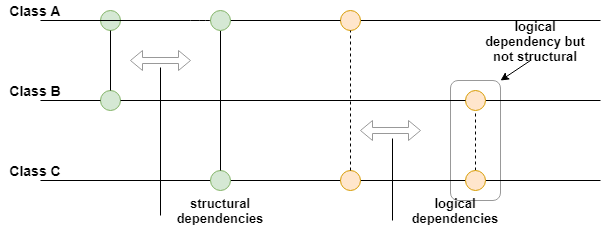
\includegraphics[scale=0.60]{fig1.png}
\caption{Relationships between structural and logical dependencies }
\label{fig:fig1}
\centering
\end{figure}




\section{Purpose of the project}
\tab A system is stable when a change in one component of the system does not affect the other components .This rule applies recursively also inside the components.
In this paper we intend to understand better the intersection between structural dependencies and logical dependencies and their impact over the system stability (Figure \ref{fig:fig2}). We also would like to study multiple ways of building and filtering logical dependencies and how this can affect the final result of the analysis.


\begin{figure}[h]
\centering
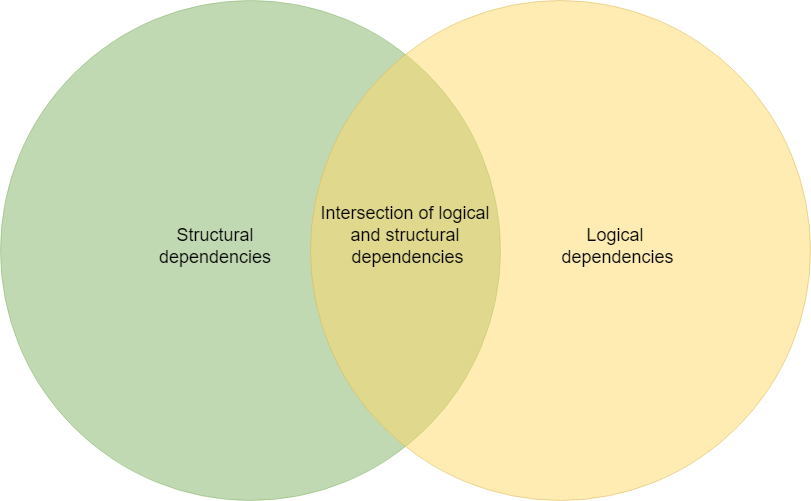
\includegraphics[scale=0.4]{fig2.png}
\caption{Venn Diagram showing the intersection between structural and logical dependencies }
\label{fig:fig2}
\end{figure}